\chapter{Implementierung}

Das folgende Kapitel beschreibt die Umsetzung der im vorherigen Kapitel beschriebenen Konzeption. Dabei wird sich sowohl bei der serverseitigen als auch clientseitigen Implementierung auf die notwendigen Schritte konzentriert, die für die Verwendung der Service Worker Technologie und die Erfüllung der Projektaufgabe erforderlich sind. Die Umsetzung der grafischen Benutzeroberfläche, Installation von MongoDB, sowie die Einrichtung der IndexedDB sind damit nicht Bestandteil dieser Dokumentation.

\section{Applicationserver}

\subsection{Node.js Express"=Server}
\label{subsec_implementierung_applicationserver}

Neben einer Datenbank bietet der Applicationserver die Funktionalitäten eines Webservers. \\
Als Backend"=Plattform wird Node.js eingesetzt und mit Hilfe von \code{Node Express} ist in wenigen Schritten ein voll"-funktionsfähiger Webserver installiert und eingerichtet. \\

\begin{lstlisting}[caption={package.json - notwendige Node.js Pakete},label={lst_realisierung_package.json}, frame=single]
{
  "name": "node-api",
  "scripts": {
    "start": "node ./bin/www"
  },
  "dependencies": {
    "bcrypt-nodejs": "0.0.3",
    "body-parser": "~1.15.2",
    "cookie-parser": "~1.4.3",
    "debug": "~2.2.0",
    "express": "~4.14.0",
    "jade": "~1.11.0",
    "jsonwebtoken": "^7.1.9",
    "mongodb": "^2.2.11",
    "mongoose": "~3.6.13",
    "morgan": "~1.7.0",
    "node-gcm": "^0.14.0",
    "passport": "^0.3.2",
    "passport-jwt": "^2.2.0"
  }
}
\end{lstlisting}


Die Bereitstellung der notwendigen Funktionalitäten setzt einige \code{node-packages} voraus, die der \code{package.json}"=Datei hinzugefügt werden (vgl. Listing \ref{lst_realisierung_package.json}). 

Wir nutzen \glqq PassportJS\grqq{} als Middleware zur Authentifizierung für Node.js und das \glqq JSON Web Token\grqq "=Prinzip für die Generierung von Authentifizierungstoken. Weiterhin werden Pakete für die Verschlüsselung von Passwörtern sowie für die Anbindung von MongoDB und \code{morgan} für das Request"=Logging installiert.

Die Umsetzung des Datenbankschemas in MongoDB sowie das objektrelationale Mapping (ORM) erfolgt mittels des \code{node-package} \code{mongoose}. Lisiting \ref{lst_a2_model-user} im Anhang \ref{subsub_a2_mongoose-schema} zeigt beispielhaft die Einrichtung der Benutzer"=Entity für die Benutzerauthentifikation. 

Eine genaue Beschreibung der Einrichtung einer Node.js"=Anwendung ist nicht Bestandteil dieser Dokumentation und soll nicht weiter beleuchtet werden. An dieser Stelle sei an zahlreiche Anleitungen im Internet verwiesen.

\subsection{Datenbank"=Server anbinden}
\label{subsec_implementierung_datenbank}

Für die persistente Speicherung der Daten auf Serverseite wird ein MongoDB"=Server aufgesetzt. Die genaue Installation und Einrichtung ist nicht Bestandteil dieser Dokumentation. \\
Nach erfolgreicher Installation muss der Applicationserver so konfiguriert werden, dass er sich mit der Datenbank verbinden und Anfragen stellen kann (vgl. Listing \ref{lst_realisierung_passport.js}).

\begin{lstlisting}[caption={Verbindung zur Datenbank konfigurieren},label={lst_realisierung_passport.js}, frame=single]
// app.js 
mongoose.connect(config.database);

// config/database.js
module.exports = {
    'secret': 'thisIsNotASecretKeyChangePlease!',
    'database': 'mongodb://localhost:27017/tasky'
};
\end{lstlisting}


\subsection{REST-Schnittstelle}

Die in Abschnitt \ref{subsec_konzeption_rest-api} geplante RESTful"=Schnittstelle wird im Node.js Express"=Server umgesetzt. Jeder Request, der sich direkt auf die Anforderung von benutzerspezifischen Ressourcen bezieht, erfordert einen gültigen Authentifizierungstoken (vgl. Anhang \ref{subsub_a2_api-security}). Es ist möglich aus dem Token den Benutzer abzuleiten und aus der Datenbank abzufragen. Wenn ein gültiger Benutzer gefunden wurde, kann das serialisierte Objekt zum eigentlichen Request hinzugefügt und die Anforderung an die entsprechende Route weitergegeben werden (\glqq Router"=Middleware\grqq).\\
Damit kann innerhalb der folgenden Routing"=Methoden direkt auf die User"=Entity zugegriffen und damit nur die Daten zu übermitteln werden, die den anfragenden Benutzer zugeordnet sind. Listing \ref{lst_realisierung_router} verdeutlicht dies beispielhaft an den \url{/api/tasks}"=Routen. In Zeile 9 bzw. Zeile 26 wird auf die User"=Entity zugegriffen, welche zuvor serverseitig aus dem JWT"=Token ausgelesen, aus der Datenbank abgefragt und dem Request hinzugefügt wurde. \\

\begin{lstlisting}[caption={Verbindung zur Datenbank konfigurieren},label={lst_realisierung_router}, frame=single]
// routes/api.js 
...
router.route('/tasks')
    // create a task (accessed from POST /api/tasks)
    .post(function(req, res){
        // create a new instance of Task model
        var task = new Task();                      
        // get user from request
        var user = req.user;                        
        // set description from the request
        task.description = req.body.description; 
        // set user   
        task.user = user._id;
        
        // save task and check for error
        task.save(function(err){
            if(err)
                res.send(err);
            res.json({ message: 'Task created!'});
        });
    })

    // get all tasks (accessed from GET /api/tasks)
    .get(function(req, res){
        var user = req.user;                  
        Task.find({ user: user._id }, function (err, tasks) {
            if(err)
                res.send(err);
            res.json(tasks);
        });
    });
...
\end{lstlisting}

\newpage
\subsubsection{Test der REST-API}

Um die Funktionalitäten der REST"=Schnittstelle zu überprüfen und zu untersuchen wird Postman\footnote{\textit{\url{https://www.getpostman.com/}}} verwendet. Dieses Tool ermöglicht es in einer grafischen Oberfläche Requests an eine URL zusammenzustellen und die entsprechenden Responses auszuwerten. \\

\begin{figure}[htp] \centering{
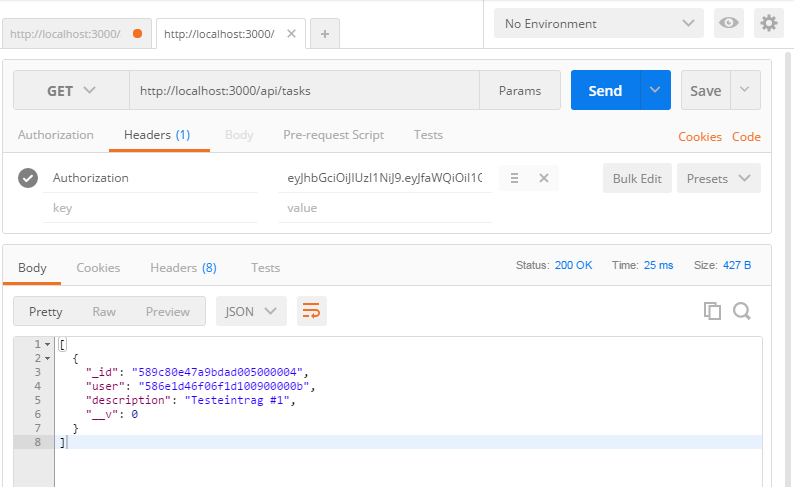
\includegraphics[width=0.85\textwidth]{images/postman.png}}
\caption{Postman: \glqq Auflistung aller Aufgaben eines authentifizierten Benutzers\grqq}
\label{image_implementierung_postman}
\end{figure} 

\newpage
\subsection{Cross-Origin Resource Sharing}

Wenn eine Webseite von einer anderen Domain, als die des Servers, Requests stellt, unterbindet normalerweise die Same"=Origin"=Policy (SOP) solche Zugriffe. Mittels Cross"=Origin Resource Sharing (CORS) ist es möglich, für bestimmte Domains derartige Anfragen an einen Server zu erlauben. 

Wir nutzen eine weitere Router"=Middleware, um allen Responses unseres Applicationsservers die in Listing \ref{lst_realisierung_router-cross-domain} aufgeführten \code{Access"=Control}"=Header hinzuzufügen. Für die Entwicklungsumgebung ist es vertretbar, sämtlichen Hosts (\code{(*)})den Zugriff zu erlauben. In einer Produktivumgebung würde man ausschließlich die Client"=Webserver"=Domain berechtigen. \\

\begin{lstlisting}[caption={Router-Middleware um jedem Response die \code{Access-Control}-Header hinzuzufügen},label={lst_realisierung_router-cross-domain}, frame=single]
router.use(function(req, res, next) {
    res.header("Access-Control-Allow-Origin", "*");
    res.header("Access-Control-Allow-Headers", "Origin, X-Requested-With, Content-Type, Accept");
    next(); // go to the next routes and don't stop here
});
\end{lstlisting}
\newpage
\section{Service Worker}
\label{sec_realisierung_serviceworker}

An dieser Stelle sei besonders erwähnt, dass die Service Worker API eine Verbindung über \code{https} erfordert. Für diese Verbindung muss ebenfalls ein gültiges Serverzertifikat vorliegen. Einzig in der Entwicklung im Umfeld von \url{localhost} ist eine unverschlüsselte Kommunikation über \url{http} möglich.

\subsection{Installation}

Um einen Service Worker zu installieren, muss dieser zuerst für die entsprechende Webseite registriert werden. Listing \ref{lst_realisierung_register-service-worker} zeigt, wie der Service Worker registriert wird.\\
Zuerst wird überprüft, ob der aktuelle Browser die Service Worker API unterstützt. Um den aktuellen Zustand des Service Workers beim Laden der Seite nachvollziehen zu können, wird dieser in die Debugging"=Konsole des Browsers geschrieben.\\
Die \code{serviceWorker.register()}"=Methode erwartet als Parameter die Service Worker Konfigurationsdatei. Diese enthält \code{Listener}, die auf verschiedene \code{Events} reagieren und die eigentliche Funktionalitäten bereitstellen. Weiterhin kann dem Service Worker ein \code{scope} übergeben werden. Dieser definiert den Context, für den die Service Worker Registration gültig ist. \\
Es ist also grundsätzlich möglich, mehrere Service Worker für eine Webanwendung zu registrieren. Jeder \code{scope} benötigt dabei eine eigene Konfigurationsdatei (diese muss sich direkt unter dem \code{scope}-Pfad befinden). Wird kein \code{scope} explizit angegeben, wird dieser aus dem Pfad der Konfigurationsdatei abgeleitet. \\

\begin{lstlisting}[caption={Einrichtung Service Worker},label={lst_realisierung_register-service-worker}, frame=single]
// js/app.js
if ('serviceWorker' in navigator)
{
    navigator.serviceWorker.register('sw.js').then(function(reg) 
    {
        if(reg.installing)
            console.log('Service worker installing');
        else if(reg.waiting)
            console.log('Service worker installed');
        else if(reg.active)
            console.log('Service worker active');
    }).catch(function(error)
    {
        // registration failed
        console.log('Registration failed with ' + error);
    });
}
\end{lstlisting}

\subsection{Caching der statischen Ressourcen}

Innerhalb der Service Worker Konfigurationsdatei wird unter anderem festgelegt, welche Ressourcen zwischengespeichert werden sollen, welche Caching"=Strategie vom Service Worker verfolgt wird und wie dieser Requests und eingehenden Responses verarbeiten soll. 

Listing \ref{lst_realisierung_sw-install} zeigt, wie die Ressourcen festzulegen sind, die im Cache vorgehalten werden. Wenn der Service Worker erfolgreich registriert wurde, wird das \code{install}"=Event ausgelöst. Für die Übersicht wurde die Liste der Ressourcen des Cache in das Array \code{urlToCache} ausgelagert. Dieses ist im Anhang \ref{subsec_a3_caching} vollständig aufgeführt.\\

\begin{lstlisting}[caption={Ressourcen festlegen, die im Zwischenspeicher vorgehalten werden sollen},label={lst_realisierung_sw-install}, frame=single]
// sw.js
this.addEventListener('install', function(event) {
    console.log('The service worker is being installed.');
    event.waitUntil( caches.open(CACHE_NAME)
        .then(function(cache) {
            return cache.addAll(urlsToCache);
        })
        .then(function(){
            return self.skipWaiting();
        })
    );
});
\end{lstlisting}
  
Die Integration des JavaScript"=\code{Promise}"=Konzepts ermöglicht es dem Service Worker im Hintergrund zu arbeiten und Anfragen asynchron zu bearbeiten. Es wird oft mit einer Verkettung von \code{Promises} gearbeitet, um auf den Abschluss einer Operation zu warten und anschließend weitere Operationen durchzuführen. Dabei kommen ebenfalls \code{callback}-Funktionen zum Einsatz, die das Ergebnis einer vorangegangenen Operation enthalten und selbst wieder einen \code{Promise} darstellen.  

\newpage
Nachdem der Service Worker erfolgreich registriert und die statischen Ressourcen für das Caching eingerichtet sind, wird die Caching"=Strategie aus Abschnitt \ref{subsec_konzept_caching-statische-ressourcen} umgesetzt. Wenn ein Request von der Webseite gestellt wird, empfängt der Service Worker \code{fetch}"=Events. Listing \ref{lst_realisierung_sw-caching} zeigt wie die Caching"=Strategie durch Verarbeitung möglicher Responses umgesetzt werden kann. \\

\begin{lstlisting}[caption={Verarbeitung empfangener Requests und Auswertung möglicher Responses im Service Worker},label={lst_realisierung_sw-caching}, frame=single]
// sw.js
this.addEventListener('fetch', function(event) {
    console.log('The service worker is serving the asset.');

    event.respondWith(
      // try to find cached resource
      caches.match(event.request).catch(function() {
        // fetch network request
        return fetch(event.request);
      }), function() { // Not fired due to the catch
        // fetch network request
        return fetch(event.request).then(function(response) {
          // save resource to cache
          return caches.open(CACHE_NAME).then(function(cache) {
            cache.put(event.request, response.clone());
            return response;
          });  
        });
      })
    );
});
\end{lstlisting}

\newpage
\subsection{Push"=Nachrichten abonnieren}

Damit eine Webanwendung Push"=Nachrichten erhalten und verarbeiten kann, benötigt sie einen aktiven Service"=Worker. Dieser kann sich mittels \code{PushManager.subscribe()} für Push"=Nachrichten anmelden. Der in Abschnitt \ref{sec_konzeption_serviceworker_architektur} beschriebene Ablauf wurde wie geplant umgesetzt. \\

\begin{lstlisting}[caption={Service Worker: Anmeldung am Push"=Server},label={lst_realisierung_sw-push-subscribe}, frame=single]
// resources/js/app.js
navigator.serviceWorker.ready.then(function(serviceWorkerRegistration) {
    serviceWorkerRegistration.pushManager.getSubscription().then(
        function(pushSubscription) {
            if(pushSubscription)
            {
                console.log("Push Subscription exists");
                // send subscription to application server
                sendSub(pushSubscription);
            }
            else
            {
                console.log("Push Subscription not existing");
                // create subscription
                subscribePush();
            }
        }.bind(this)).catch(function(e) {
        console.error('Error getting subscription', e);
    });
});
\end{lstlisting}

Nachdem geprüft wurde, ob für den aktiven Service Worker bereits eine \code{PushSubscription} vorhanden ist (siehe Listing \ref{lst_realisierung_sw-push-subscribe}), wird entweder die \code{PushSubscription} an den Applicationserver übertragen (\code{sendSub()}"=Funktion) oder eine Anmeldung beim Push"=Service innerhalb der Methode \code{subscribePush()}) initiiert. 
Nach erfolgreicher Anmeldung mittels \code{PushManager.subscribe()} wird die zurückgegebene \code{PushSubscription} mit Hilfe der Funktion \code{sendSub()} an den Applicationserver übertragen. Im Anhang \ref{sec_a3_sw-push-functions} sind die Funktionen für die Anmeldung, Abmeldung und Übertragung der \code{PushSubscription} aufgeführt.

\newpage
\subsubsection{Endpoint auf Applicationserver speichern}

Die im Anhang \ref{sec_a3_sw-push-functions} aufgeführte \code{sendSub()}"=Funktion ist dafür verantwortlich, die Endpoint"=Informationen auf den Applicationserver zu übertragen. \\
Neben dem Endpoint und der Subscription"=ID wird eine eindeutige \code{DeviceID} sowie ein optionaler Gerätename übertragen. 

Der Applicationserver speichert diese Informationen in der Datenbank bzw. aktualisiert einen bereits vorhandenen \code{Device}"=Eintrag für den entsprechenden Benutzer und der \code{DeviceID}. Die \code{DeviceID} wird mit Hilfe der \code{Fingerprint2}"=Bibliothek\footnote{\textit{\url{https://github.com/Valve/fingerprintjs2}}} generiert und ist für jedes Gerät und Browser eindeutig. \\ 

\begin{lstlisting}[caption={Bei Seitenstart prüfen, ob eine DeviceID vorhanden ist und ggf. anlegen},label={lst_realisierung_deviceId}, frame=single]
// CHECK if unique device id exists
$(document).ready(function(){

    // store device id
    var deviceId = localStorage.getItem("deviceId");
    if(deviceId === null)
    {
        new Fingerprint2().get(function(result, components){
            localStorage.setItem("deviceId", result);
            console.log("Set deviceId: " + result); //a hash, representing your device fingerprint
        });
    }
    console.log("DeviceID: " + deviceId);
});
\end{lstlisting}

\subsubsection{Verarbeitung von \code{Push}-Events}

Wenn der Service Worker eine Push"=Nachricht empfängt, wird das Event \code{push} ausgelöst. In der Service Worker Konfigurationsdatei wird dafür ein \code{EventListener} registriert. Listing \ref{lst_realisierung_push-event-listener} zeigt, wie bei eintreffenden Push"=Benachrichtigungen beim Applicationserver der zugehörige Payload angefragt wird. \\
Wenn der empfangene Payload den Type \code{update} trägt, bedeutet dies, dass sich im \code{body} Aktualisierungen des Models verbergen. Daraufhin wird die Funktion \code{updateIndexedDb()} aufgerufen. Als Parameter erwartet diese ein mehrdimensionales Array aus serialisierten Objekten. Diese sind mit einem Timestamp versehen und werden ggf. in der lokalen Datenbank aktualisiert. \\

\begin{lstlisting}[caption={Service Worker \code{push}"=EventListener},label={lst_realisierung_push-event-listener}, frame=single]
// sw.js
self.addEventListener('push', function(event) {
    console.log('Push message', event);

    event.waitUntil(getEndpoint().then(function(endpoint){
        var subId = endpoint.split("/").pop();
        var request = new Request(PUSH_URL + "/payload/"+subId, {
            method: 'GET',
            mode: 'cors',
            redirect: 'follow'
        });
        return fetch(request);
    }).then(function(res) {
        res.json().then(function(data){
            if(data.type == "update")
            {
                updateIndexedDb(data.body);
            }
            else
            {
                // Show notification
                self.registration.showNotification(data.title, {
                    'body': data.body,
                    'icon': data.icon
                });
            }
            console.log(data);
        })
    });
});
\end{lstlisting}

In dem Fall, dass der Payload nicht den Typ \code{update} trägt, wird davon ausgegangen, dass eine \code{Push"=Notification} angezeigt werden soll. Der Payload enthält die notwendigen Attribute, um eine Benachrichtigung anzuzeigen (vgl. Abbildung \ref{image_implementierung_notification}). Benachrichtigungen werden sowohl auf mobilen Endgeräten als auch auf Desktop"=PC`s angezeigt. \\

\begin{figure}[htp] \centering{

\includegraphics[width=0.4\textwidth]{images/notification.png}}
\caption{Beispiel Anzeige einer Desktop"=Benachrichtigung}
\label{image_implementierung_notification}
\end{figure} 

\newpage
\subsection{Background Sync}
\label{subsec_implementierung_background-sync}

Ähnlich der Push"=Benachrichtigung verwendet Background Sync den Service Worker als Event"=Target. Dadurch können Synchronisationen durchgeführt werden, obwohl die betroffene Webseite nicht geöffnet ist oder gerade keine aktive Internetverbindung besteht. Um diese Funktionalität verwenden zu können, muss ein \code{sync} beim Service Worker registriert werden. \\

\begin{lstlisting}[caption={Registrierung Background Sync},label={lst_realisierung_register-background-sync}, frame=single]
// js/app.js
if ('serviceWorker' in navigator && 'SyncManager' in window) 
{
  navigator.serviceWorker.ready.then(function(reg) {
    return reg.sync.register('appStateSync');
  }).catch(function() {
    // system was unable to register for a sync,
    // this could be an OS-level restriction
    postDataToServer();
  });
}
else 
{
  // serviceworker/sync not supported
  postDataToServer();
}
\end{lstlisting}

Da nicht alle Browser die Background"=Sync"=Funktionalitäten unterstützen, jedoch Service Worker teilweise integriert haben, bietet es sich an eine erweiterte Prüfung durchzuführen. Listing \ref{lst_realisierung_register-background-sync} zeigt, wie neben der Service Worker Unterstützung auf Background Sync Funktionalität geprüft wird. \\
Die Funktion \code{postDataToServer()} bildet den Fallback, falls Background Sync nicht unterstützt wird, und überträgt die Zustandsdaten über \glqq klassische\grqq{} Verfahren (vor Background Sync) mittels AJAX"=Requests.\\

\begin{lstlisting}[caption={\code{sync}"=EventListener in der Service Worker Konfigurationsdatei},label={lst_realisierung_sw-background-sync}, frame=single]
// sw.js
this.addEventListener('sync', function(event) 
{
  if (event.tag == 'appStateSync') 
    event.waitUntil(syncLocalDatabase());
});
\end{lstlisting}

Die Funktion \code{syncLocalDatabase()} synchronisiert die locale IndexedDB mit der Datenbank des Applicationserver. Dabei werden ausschließlich Daten lokal im Client gespeichert, die für den Benutzer relevant sind. Die Funktion gibt einen \code{Promise} zurück, so dass die Synchronisation asynchron im Hintergrund ausgeführt werden kann. \\
Bei jedem Sync wird der aktuelle Timestamp in einem gesonderten \code{STORE} (dieser enthält ebenfalls weitere Konfigurationsparameter) gespeichert und nur diejenigen Daten vom Applicationserver angefordert, die sich seit der letzten Aktualisierung geändert haben. Anschließend werden diese Objekte durchlaufen und der Timestamp der letzten Änderung mit der letzten Änderung des lokal hinterlegten Objekts verglichen und ggf. wird der Eintrag aktualisiert.

Schlägt die Synchronisation fehl, wird diese automatisch vom Background Sync Dienst wiederholt (durch erneuten auslösen eines \code{sync}"=Events).